\section{Experimental Setup}
\label{sec:setup}

\subsection{Azerbaijani task data}
\label{sec:setup:data}
The Azerbaijani source is the LocalDoc sentiment dataset on Hugging Face \cite{localdoc2024sentiment} (42{,}000 texts from social networks and reviews, three classes, licence CC-BY-NC-SA-4.0). The dataset exceeds the brief's floor of 10{,}000 labelled examples; the primary cells at $n\in\{500,2{,}000\}$ are deliberate low-resource subsamples of a fixed training split, chosen because that is where transfer effects are expected and where escape instability was measured in pilots, and the full-size cell $n=20{,}914$ establishes the ceiling. Table~\ref{tab:azdata} traces the pipeline. Neutral examples are removed to obtain a binary task; label-aware exact-text deduplication removes 86 duplicates (0.31\%) with zero label conflicts, \emph{before} a stratified split with seed 12{,}345. The resulting splits are balanced, and an exact-text leakage check finds no overlap between any pair of splits. Because the upstream Hugging Face revision is not pinned, an order-invariant content manifest (SHA-256 over sorted normalised text–label pairs) is recorded for every split; the supplied \file{data.tgz} snapshot is the only exact copy of the data the grid saw, and any reproduction must verify the manifests before treating a fresh download as equivalent. No scraping was performed and no personal data beyond the public dataset was used.

\begin{table}[!t]
\caption{Azerbaijani data pipeline and splits (\file{results/splits.json}). The pre-grid characterisation package (Section~\ref{sec:setup:audit}) used 20{,}936/2{,}791/4{,}187 and carries no manifest.}
\label{tab:azdata}
\centering
\scriptsize
\begin{tabular}{@{}L{5.3cm}R{3.3cm}@{}}
\toprule
Step & Count \\
\midrule
Upstream rows (positive / neutral / negative) & 42{,}000 \\
After removing \pfx{neutral} & 28{,}000 \\
After label-aware exact-text deduplication (86 removed, 0 conflicts) & 27{,}914 \\
Train / validation / test (stratified, seed 12{,}345) & 20{,}937 / 2{,}791 / 4{,}186 \\
Train label distribution (negative / positive) & 10{,}472 / 10{,}465 \\
Test label distribution (negative / positive) & 2{,}094 / 2{,}092 \\
Exact-text leakage train–test / train–val / val–test & 0 / 0 / 0 \\
Content manifest, test split (SHA-256 prefix) & \pfx{ca19c0bb} \\
Content manifest, validation / train (prefix) & \pfx{5cd479fb} / \pfx{d1cf165c} \\
Upstream revision pinned & no \\
\bottomrule
\end{tabular}
\end{table}

\subsection{Human label audit (pre-grid)}
\label{sec:setup:audit}
Two annotators independently labelled 100 examples sampled under the pre-grid split (Table~\ref{tab:audit}). Three-class human–human agreement is 66/99 (66.67\%, $\kappa=0.491$). Among rows retained by the binary task, the \emph{unconditioned} agreement is 44/67 (65.67\%); the higher 37/42 (88.10\%, $\kappa=0.746$) conditions on both humans and the dataset all committing to a polarity and therefore selects easier examples. The unconditioned figure is the relevant disclosure of retained-label quality, and the two annotators are not interchangeable (68.66\% vs.\ 59.70\% against gold). Because the pre-grid split differs from the grid split by one example and has no manifest, these numbers characterise the dataset, not the specific holdout.

\begin{table}[!t]
\caption{Human label audit, 100 sampled examples (\file{evidence/carried\_forward\_pre\_grid/}).}
\label{tab:audit}
\centering
\scriptsize
\begin{tabular}{@{}L{4.5cm}R{4.1cm}@{}}
\toprule
Quantity & Value \\
\midrule
Three-class human–human agreement & 66/99 = 66.67\% ($\kappa$ = 0.491) \\
Human–human on retained polar rows, unconditioned & 44/67 = 65.67\% \\
Human–human, all three sources commit to a polarity & 37/42 = 88.10\% ($\kappa$ = 0.746) \\
Annotator 1 vs.\ gold (100 / retained 67) & 71.0\% / 68.66\% \\
Annotator 2 vs.\ gold (100 / retained 67) & 58.59\% / 59.70\% \\
Audit verdict & \pfx{PROCEED\_WITH\_CAVEAT} \\
\bottomrule
\end{tabular}
\end{table}

\subsection{Turkish source data}
TRSAv1 \cite{aydogan2023trsav1} provides 150{,}000 Turkish e-commerce reviews with three labels; the captured dataset card declares no licence. Label-aware deduplication removes 11{,}360 rows (7.57\%; 937 texts had conflicting labels), leaving 138{,}640, from which a seeded, label-stratified subsample of 20{,}000 is deterministically partitioned into 18{,}000 source-training and 2{,}000 source-validation examples. The shuffled corpus is derived from the same 20{,}000 (Section~\ref{sec:method:turkish}).

\subsection{Pre-registration and amendments}
\label{sec:setup:prereg}
The experimental specification was frozen on 4 September 2026 and hash-locked (\file{configs/CONFIG\_HASHES.lock}); every later change is an amendment recorded with its date and rationale before the affected runs (Table~\ref{tab:prereg}). Two classes of amendment exist. Non-scientific execution changes (validation cadence 65$\to$200 steps, evaluation batch size, two-phase execution, a gradient-accumulation option adopted and then reverted before any run completed) do not alter what the optimizer does at any step. Amendments~6 and~8, written before the final grid, repair defects found by a forensic audit of an earlier 114-run grid: validation-selected checkpoint restoration with numerical verification, a genuinely reset task head, a well-defined mean placebo, UNK-free anchors, degeneracy accounting, dual estimands with family-wise correction, and content manifests. That earlier grid is retained unmodified as a separate artefact and is not pooled with the 164 runs reported here. The escape threshold $\theta=0.40$, the seeds, sizes, $k$, $m$, and every optimizer setting were never changed after the freeze.

\begin{table}[!t]
\caption{Pre-registration timeline (\file{evidence/preregistration/FROZEN.md}).}
\label{tab:prereg}
\centering
\scriptsize
\begin{tabular}{@{}L{1.4cm}L{7.1cm}@{}}
\toprule
Date (2026) & Event \\
\midrule
04 Sep & Specification frozen; hash lock; $\theta=0.40$ fixed from pilots \\
04 Sep & Validation cadence 65 $\to$ 200 steps; eval batch size; A100/H100 migration notes; gradient accumulation $8\times4$ authorised \\
05 Sep & Accumulation reverted to pre-registered batch 32 $\times$ 1 (no run had completed under $8\times4$) \\
06 Sep & 114-run validation-only grid (retained separately, not pooled) \\
07 Sep & Amendments 1–5: Turkish conditions and contrast base at $n=500$; test split spent once with ledger; schema v4; per-method C1c provenance \\
07 Sep & Amendment 6: best-validation checkpoint restore with $10^{-4}$ verification \\
08 Sep & Amendment 8: nearest-$k$ mean placebo; UNK/special rejection in anchors; full task-head reset; degeneracy accounting; all-seed estimand, paired tests, Holm; manifests; valid JSON \\
08–09 Sep & Final 164-run grid executed (19:39 UTC 8 Sep to 03:58 UTC 9 Sep) \\
\bottomrule
\end{tabular}
\end{table}

\subsection{Grid, seeds, and hyperparameters}
\label{sec:setup:grid}
Table~\ref{tab:hparams} lists the frozen values. At $n=500$ and $n=2{,}000$ both encoders run all seven conditions with seeds $\{42, 1337, 13, 7, 2024\}$ (140 runs); \xlmxv{} additionally runs the four non-Turkish conditions at $n\in\{10{,}000, 20{,}914\}$ with seeds $\{42, 1337, 13\}$ (24 runs). The launcher records 164 requested, 164 completed, zero failures, and no skipped-existing records. The queue is ordered reference-size-first so that a truncated window would still yield a complete comparison table.

\begin{table}[!t]
\caption{Frozen hyperparameters and grid composition (\file{configs/experiment.yaml}, \file{FROZEN.md}).}
\label{tab:hparams}
\centering
\scriptsize
\begin{tabular}{@{}L{3.0cm}L{5.5cm}@{}}
\toprule
Setting & Value \\
\midrule
Azerbaijani budget & 2{,}000 optimizer steps (all $n$) \\
Batch / accumulation / effective batch & 32 / 1 / 32 \\
Optimizer & AdamW \cite{loshchilov2019adamw}, lr $2\times10^{-5}$, warm-up 10\%, weight decay 0.01 \\
Precision / max length / padding & fp16 AMP / 256 / dynamic \\
Validation cadence & every 200 steps (10 points incl.\ terminal) \\
Selection rule & max validation \Fone, ties $\to$ lower step; restore and verify ($10^{-4}$) \\
Early stopping & disabled \\
Escape threshold $\theta$ & 0.40 (fixed from pilots, hash-locked) \\
Turkish stage & 2 epochs, 18k train / 2k val, 3 labels, cached (30 checkpoints) \\
Transplant & functional anchors; $k=64$; $m=256$; rescale to anchor median; transplant seed 0 \\
Seeds ($n\le2{,}000$ / $n>2{,}000$) & \{42, 1337, 13, 7, 2024\} / \{42, 1337, 13\} \\
Split seed & 12{,}345 \\
Runs: $2\times7\times2\times5$ + $1\times4\times2\times3$ & 140 + 24 = 164 (164 completed, 0 failed) \\
Determinism & \pfx{use\_deterministic\_algorithms}; cuDNN deterministic \\
\bottomrule
\end{tabular}
\end{table}

\subsection{Test-split protocol and disclosures}
\label{sec:setup:test}
The inference family is defined on validation. The test split is evaluated once per run, only at the restored validation-selected checkpoint, and only after the restore has been numerically verified; the ledger \file{results/test\_evaluation\_ledger.jsonl} holds exactly 164 entries, one per completed run, all from the single call site \file{finetune.run\_single}, which defaults to the validation split and evaluates the test split only with an explicit opt-in flag. No model, step, hyperparameter, or condition was selected using a test number; test-side statements in Section~\ref{sec:results} are confirmations of validation-selected claims (Section~\ref{sec:method:stats}).

\subsection{Compute environment and budget}
\label{sec:setup:compute}
The 164-run grid executed on a rented instance with one NVIDIA H100 NVL (95{,}830~MiB), an AMD EPYC 9V84 (40 vCPU), 313~GiB RAM, driver 595.71 with CUDA 13.2 host and PyTorch 2.11.0+cu128, in a single stream throughout (\pfx{streams\_active}\,$=1$ in all 164 records). Table~\ref{tab:compute} summarises cost: 8.36 process-hours summed over runs, of which 8.02~h is the Azerbaijani stage; launcher wall-clock 8.37~h; roughly 9.5~h including the serial Turkish-cache phase; hence about 9.5 device-hours. Per-run wall-clock is 2.5–6.8 minutes (Fig.~\ref{fig:runtime}). This is far inside the brief's two-day training envelope. Peak GPU memory during the grid is \NM: the launcher's memory sampler did not run, no run record carries a maximum allocation, and the 97~MiB reading captured after completion describes an idle device. A 30-step benchmark at the locked batch and sequence settings on a different, pre-grid machine (RTX 4060 laptop, 8.59~GB) measured 8.6~GB peak reserved memory; we report it as a labelled pre-grid measurement on other hardware, not as the grid's footprint, and note that a stream ceiling of 10~GB was enforced by the launcher configuration on every venue.

\begin{table}[!t]
\caption{Compute cost of the final grid (\file{evidence/environment/ENVIRONMENT\_AS\_RUN.md}, \file{results/aggregate.csv}, \file{results/launcher\_state.json}). Per-run wall-clock in minutes.}
\label{tab:compute}
\centering
\scriptsize
\begin{tabular}{@{}lrrrrr@{}}
\toprule
Base & Runs & Process-h & Mean & Min & Max \\
\midrule
% AUTO-GENERATED by report/ieee/tables/make_tables.py -- do not edit by hand.
% source: results/aggregate.csv
% source: results/launcher_state.json
XLM-15 & 94 & 5.00 & 3.19 & 2.94 & 3.60 \\
XLM-R & 70 & 3.36 & 2.88 & 2.53 & 6.77 \\
\midrule
All & 164 & 8.36 & 3.06 & 2.53 & 6.77 \\
\bottomrule

\end{tabular}
\par\smallskip
\begin{minipage}{\columnwidth}\footnotesize
Azerbaijani-stage process-hours: 8.02; launcher elapsed: 8.37 h; streams: 1. Wall-clock incl.\ the serial Turkish-cache phase $\approx$ 9.5 h $\Rightarrow$ $\approx$ 9.5 GPU-hours on one GPU. Peak GPU memory during the grid: \NM{} (sampler did not run). Pre-grid 30-step benchmark on an RTX 4060 at the same batch and length: 8.6 GB peak reserved.
\end{minipage}
\end{table}

\begin{figure}[!t]
\centering
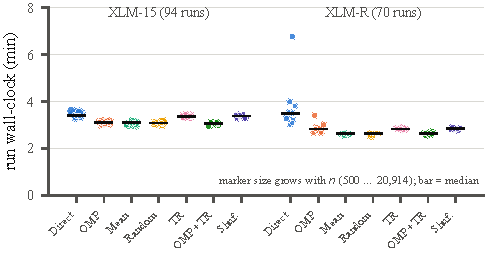
\includegraphics[width=\columnwidth]{figures/fig_runtime.pdf}
\caption{Per-run wall-clock by base and condition, all 164 runs (\file{results/aggregate.csv}). Marker size grows with $n$; the bar is the cell median. Turkish-bearing runs exclude the cached source stage.}
\label{fig:runtime}
\end{figure}

\subsection{Software stack and reproducibility}
\label{sec:setup:repro}
The executed environment used Python 3.12.14, PyTorch 2.11.0+cu128 \cite{paszke2019pytorch}, Transformers 4.57.6 \cite{wolf2020transformers}, Tokenizers 0.22.2, Datasets 5.0.1, NumPy 2.5.3, SciPy 1.18.1, scikit-learn 1.9.0 \cite{pedregosa2011sklearn}, pandas 3.0.5 and Matplotlib 3.11.1 (Table~\ref{tab:stack}). Two disclosures follow from the environment capture. The pre-run \file{requirements.lock} was unresolvable on the host because of a Datasets/fsspec conflict, so it did not describe the run; \pfx{sacremoses} (needed by the \xlmxv{} tokenizer) and \pfx{protobuf} (needed for SentencePiece conversion) were undeclared and installed after import failures. \file{requirements.txt} and \file{requirements.lock} were regenerated from the post-run freeze and describe the environment the reported numbers were computed on; they do not retroactively prove that the original specification was sufficient.

\begin{table}[!t]
\caption{Pre-run pins vs.\ the stack that actually ran (\file{evidence/environment/}).}
\label{tab:stack}
\centering
\scriptsize
\begin{tabular}{@{}lll@{}}
\toprule
Package & Pre-run lock & As run \\
\midrule
torch & 2.4.1+cu121 & 2.11.0+cu128 \\
transformers & 4.44.2 & 4.57.6 \\
tokenizers & 0.19.1 & 0.22.2 \\
datasets & 2.21.0 & 5.0.1 \\
numpy & 1.26.4 & 2.5.3 \\
scipy & 1.14.1 & 1.18.1 \\
scikit-learn & 1.5.2 & 1.9.0 \\
pandas & 2.2.3 & 3.0.5 \\
matplotlib & 3.9.2 & 3.11.1 \\
sentencepiece & 0.2.0 & 0.2.2 \\
sacremoses & 0.2.0 & 0.2.0 (undeclared) \\
protobuf & absent & 7.36.1 (undeclared) \\
\bottomrule
\end{tabular}
\end{table}

All seeds, sizes, paths and analysis rules are read from \file{configs/experiment.yaml}; \file{run\_all.sh} is the single entry point that rebuilds anchors, transplants, controls, the Turkish cache, the 164-run grid, and the aggregate, statistics, and table files in order, with automatic resume through \pfx{skip\_existing}. The repository's continuous-integration workflow (\file{.github/workflows/ci.yml}) runs the CPU unit-test suite (\pfx{pytest -m 'not slow'}, offline, no model or dataset downloads) together with repository-hygiene checks on every push to and pull request against \pfx{main}. Every result file cited in this paper is committed: 164 schema-v4 run records (each with the ten-point validation history, the training-loss history, the test block with all 4{,}186 predictions, the selection and restoration fields, and the task-head-reset and source-stage metadata), the per-run logs, \file{aggregate.csv}, \file{summary.csv}, \file{stats.csv}, the intrinsic-diagnostic and control files, the environment captures, and the pre-registration documents (Appendix~\ref{app:evidence}). Per-run model weights and the 30 Turkish-stage checkpoints are not distributed (tens of GB); their reconstruction costs roughly 2.5 GPU-hours.
